\documentclass{article}
\usepackage[utf8]{inputenc}
\usepackage{amsmath}
\usepackage{setspace}
\usepackage{mathtools}
\usepackage{amssymb}
\usepackage{amsfonts}
\newcommand\der[2]{\frac{\partial{#1}}{\partial{#2}}}
\usepackage{sectsty}
\usepackage[parfill]{parskip}
\usepackage{changepage}   % for the adjustwidth environment
\usepackage{graphicx}
\graphicspath{ {./Pictures/} }
\usepackage{float}
\usepackage[margin=1in]{geometry}
\setlength{\parindent}{0em}
\sectionfont{\fontsize{12}{12}\selectfont}
\nonfrenchspacing
\renewcommand{\baselinestretch}{1.5}
\usepackage{indentfirst}
\usepackage{enumitem}
\setlist[itemize]{topsep=0pt,itemsep=0pt,partopsep=0pt,parsep=0pt}
\usepackage{xcolor}
\usepackage{titlesec}
\DeclareUnicodeCharacter{2212}{-}
\usepackage{tikz}
\usetikzlibrary{calc}
\newcommand{\tikzmark}[1]{\tikz[overlay,remember picture] \node (#1) {};}
\titleformat{\section}[block]{\color{blue}\Large\bfseries\filcenter}{}{1em}{}
\usepackage[normalem]{ulem}
\usepackage{calrsfs}
\renewcommand{\labelitemiv}{$\circledast$}
\renewcommand{\labelitemii}{$\circ$}
\titlespacing*{\subsubsection}{0pt}{0ex}{0ex}
\setlength{\parskip}{0.6em}

\title{ECON3510 Formula Sheet}
\date{2019}

\begin{document}

\maketitle

\section{Symbols}
$^{*}$ refers to foreign \\
$\text{variable}_{1},\text{variable}_{2}$ refers to goods $1$ and $2$ \\
$a_{i}$ refers to labor hours required to produce good i \\
$\text{variable}^{w}$ refers to world \\
$s$ refers to specialized good \\
$w$ refers to wage \\
$r$ refers to rental rate for capital \\
$PFQ$ refers to the production function of Q \\

\newpage

\section{Ricardian Equations in Terms of Home}
\underline{Gravity Model}: $T_{i,j} = \frac{A \times Y_{i} \times Y_{j}}{D_{i,j}}$ \\
\underline{Wage}: $w_{1} = \frac{P_{1}}{a_{1}}$ \\
\underline{Relative Wage}: $\frac{w}{w^{*}} = \frac{P_{1}}{a_{1}} \div \frac{P_{2}}{a_{2}^{*}} = \frac{P_{1}}{a_{1}} \cdot  \frac{a_{2}^{*}}{P_{2}}$ \\
\underline{Real Wages without Trade}: $w_{1}^{r} = \frac{w_{1}}{p_{1}} = \frac{1}{a_{1}}$
\begin{itemize}
  \item  \underline{Note}: this is equivalent to MPL
\end{itemize}
\underline{Real Wages with Trade}: $w_{1}^{r1} = \frac{w_{1}}{P_{1}^{w}} = \frac{1}{a_{1}}$ wages for good 1 in terms of specialized good 1, $w_{1}^{r2} = \frac{w_{1}}{P_{2}^{w}} = \frac{1}{a_{1}} \times \frac{P_{1}^{w}}{P_{2}^{w}}$ wages for good 1 in terms of non-specialized good 2
\begin{itemize}
  \item  \underline{Note}: make sure to use world prices
  \item  \underline{Derivation of Real Wages for Good 1 in Terms of Non-Specialized Good 2}: we have that $w_{1}^{r2} = \tfrac{w_{1}}{p_{2}^{w}}$, however we do not typically know the value of $p_{2}^{w}$. Instead, we usually only know the world price ratio $\tfrac{p_{1}^{w}}{p_{2}^{w}}$ is and so we need to find a solution for $w_{1}^{r2}$ in terms of $\tfrac{p_{1}^{w}}{p_{2}^{w}}$. Note that if we multiply both sides of our equation for $w_{1}^{r2}$ by $\tfrac{p_{1}^{w}}{p_{1}^{w}}$ we get:
  \begin{align*}
    w_{1}^{r2} &= \frac{w_{1}}{p_{2}^{w}} \cdot \frac{p_{1}^{w}}{p_{1}^{w}} \\
    w_{1}^{r2} &= \frac{w_{1}}{p_{1}^{w}} \cdot \frac{p_{1}^{w}}{p_{2}^{w}} \ \tag{*}
  \end{align*}
  Further note that from our equation for $w_{1}^{r1}$ we know that $\tfrac{w_{1}}{p_{1}^{w}} = \tfrac{1}{a_{1}}$. Inserting this into equation (*) yields the following soluton for real wages in terms of non-specialized good 2:
  \begin{gather*}
    w_{1}^{r2} = \frac{1}{a_{1}} \times \frac{p_{1}^{w}}{p_{2}^{w}}
  \end{gather*}
\end{itemize}
\underline{Relative Productivity}: $\frac{a_{1}}{a_{1}^{*}}$ \\
\underline{Marginal Rate of Substitution}: $MRS_{1,2} = \frac{MU_{1}}{MU_{2}} = \frac{P_{1}}{P_{2}}$ \\
\underline{Production}: $a_{1}Q_{1} + a_{2}Q_{2} = L$ \\
\underline{Production Possibility Frontier}: $Q_{1} = \frac{L}{a_{1}} - \frac{a_{2}}{a_{1}}Q_{2}$ \\
\underline{Marginal Productivity of Labor}: $MPL_{1} = \frac{1}{a_{1}}$ \\
\underline{Opportunity Cost}: $OC_{1} = \frac{a_{1}}{a_{2}}$ \\
\underline{Relative Price in Autarky}: $\frac{P_{1}}{P_{2}} = \frac{a_{1}}{a_{2}}$ \\
\underline{Relative Price in Free Trade}: $\frac{P_{1}}{P_{2}} = \frac{\text{total} \ Q_{1}}{\text{total} \ Q_{2}}$ where the quantity is the total produced in the economy \\
\underline{Autarky Equilibrium Occurs When}: $\frac{P_{1}}{P_{2}} = \frac{a_{1}}{a_{2}} = MRS_{1,2}$ \\
\underline{Closed Trade Specialization of Good 1 Occurs When}: $w_{1} = \frac{P_{1}}{a_{1}} > \frac{P_{2}}{a_{2}} = w_{2} \Rightarrow \frac{P_{1}}{P_{2}} > \frac{a_{1}}{a_{2}}$ \\
\underline{Free Trade Specialization of Good 1 (World Price is Not Given) Occurs When}:
 \begin{gather*}
   \frac{a_{1}}{a_{2}} < \frac{a_{1}^{*}}{a_{2}^{*}} \equiv wa_{1} < w^{*}a_{1}^{*} \equiv \frac{a_{1}^{*}}{a_{1}} > \frac{w}{w^{*}}
 \end{gather*}
\underline{Free Trade Specialization with World Price Given (three cases)}:
\begin{itemize}
  \item  \underline{Case 1}: $\frac{P_{1}}{P_{2}} = \frac{a_{1}}{a_{2}} < \frac{a_{1}^{*}}{a_{2}^{*}}$ then foreign specializes in good 2 and home does not specialize
  \item  \underline{Case 2}: $\frac{P_{1}}{P_{2}} < \frac{a_{1}}{a_{2}} < \frac{a_{1}^{*}}{a_{2}^{*}}$ then both home and foreign specialize in good 2
  \item  \underline{Case 3}: $\frac{a_{1}}{a_{2}} < \frac{P_{1}}{P_{2}} < \frac{a_{1}^{*}}{a_{2}^{*}}$ then home specializes in good 1 and foreign specializes in good 2
\end{itemize}

\newpage

\section{Heckscher-Ohlin Model}
\underline{Production Possibility Frontier}: $L = f(Q_{1}, Q_{2})$ \\
\underline{Isovalue Line - Representing Constant Value of Production (Indifference Curves)}: $V = P_{1}Q_{1} + P_{2}Q_{2}$
\begin{itemize}
  \item  \underline{Slope}: $-\tfrac{P_{1}}{P_{2}}$
\end{itemize}
\underline{Production}: occurs at the intersection of the most north-eastern isovalue line and the PPF, i.e. where $P_{C}/P_{F}$ equals the slop of the PPF  \\
\underline{MRS and Relative Price}: $P_{1}/P_{2} = \text{MRS}_{1,2}$ \\
\underline{Isoquant}: represents input possibilities in food production, where capital and labor inputs are imperfectly substitutible  \\
\underline{Relative Labor/Capital Demand}: if $\tfrac{L_{1}}{K_{1}} >  \tfrac{L_{2}}{K_{2}}$ then production of $1$ is relatively labor intensive and production of $2$ is relatively capital intensive
\begin{itemize}
  \item  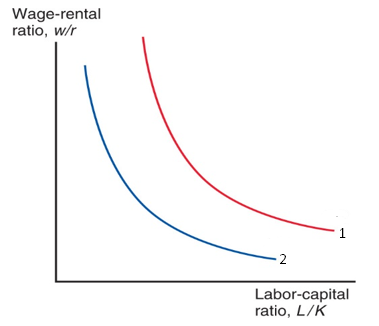
\includegraphics[width=4cm, height=4cm]{pic1}
  \item  At any given wage/rental-ratio, production of 1 uses a higher labor-capital ratio since 1 is labor intensive and 2 is capital intensive
\end{itemize}
\underline{Wage Rental Ratio}: $\tfrac{w}{r}$
\begin{itemize}
  \item  \underline{Note}: changes in $\tfrac{w}{r}$ are tied to changes in $\tfrac{P_{1}}{P_{2}}$  \\
  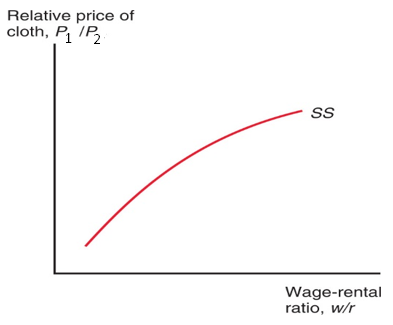
\includegraphics[width=4cm, height=4cm]{pic2}
\end{itemize}
\underline{Stolper-Samuelson Theorem}: if the relative price of a good increases, then the real wage or rental rate of the factor used intensively in the production of that good increases, while the real wage or rental rate of the other factor decreases. Thus any change in the relative price of goods alters the distribution of income.
\begin{itemize}
  \item  \underline{Note}: if the relative price of cloth rises, the wage-rental ratio must rise. This will cause the labor-capital ratio used in the production of both goods to drop \\
  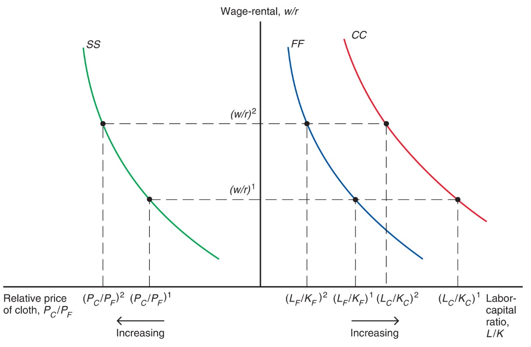
\includegraphics[width=6cm, height=4cm]{pic3}
\end{itemize}
\underline{Increase in Relative Price Effect} if the relative price for good 1 $P_{1}/P_{2}$ increase then this will:
\begin{itemize}
  \item  \underline{(1)}: raise income of workers relative to that of capital owners, $\tfrac{w}{r}$
  \item  \underline{(2)}: raise the ratio of capital to labor services, $\tfrac{K}{L}$ used in both industries
  \item  \underline{(3)}: raise the real income (purchasing power) of workers and lower the real income of capital owners
  \item  \underline{(4)}: raises the purchasing power of labor in terms of both goods while lowers the purchasing power of capital in terms of both goods
\end{itemize}
\underline{Rybczynski Theorem}: holding output prices constant, as the amount of a factor of production increases, the supply of the good that uses this factor intensively increases and the supply of the other good decreases
\begin{itemize}
  \item  \underline{Example}: an increase in the supply of labor shifts the economy’s production possibility frontier outward disproportionately in the direction of the more labour intense good's (cloth) production. At an unchanged  of cloth, the less labour intense good's (food) production declines \\
  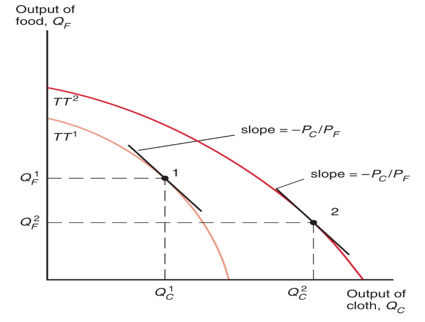
\includegraphics[width=8cm, height=6cm]{pic4}
\end{itemize}
\underline{Trade Convergence}: trade leads to a convergence of s
\begin{itemize}
  \item  \underline{Example}: in the absence of trade, Home’s equilibrium would be at point 1, where domestic relative supply RS intersects the relative demand curve RD. Similarly, Foreign’s equilibrium would be at point 3. Trade leads to a world  that lies between the pretrade prices, such as at point 2 \\
  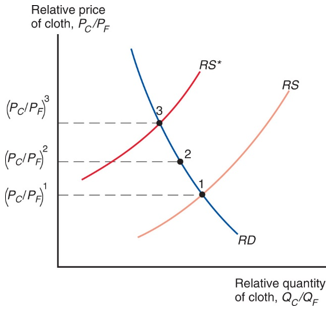
\includegraphics[width=8cm, height=6cm]{pic5}
\end{itemize}
\underline{Heckscher-Ohlin Theorem}: the country that is abundant in a factor exports the good whose production is intensive in that factors, so countries tend to export goods whose production is invensive in factors with which countries are abundantly endowed \\
\underline{Relative Consumption of Home}: $(Q_{1}-X_{1})/(Q_{2}-X_{2})$ \\
\underline{Relative Consumption of Foreign}: $(Q_{1}^{*}+X_{1})/(Q_{2}^{*}+X_{2})$ \\
\underline{Optimality Condition under Autarchy}: optimality under autarchy requires each countries  of good 1 to equal it's opportunity cost of production of good 1 and the marginal rate of substitution in consumption of good 1, so we have three conditions:
\begin{align*}
  \textit{Optimality in Production: }& \tfrac{P_{1}}{P_{2}} = f_{OC}(\tfrac{Q_{1}}{Q_{f}}) \\
  \textit{Optimality in Consumption: }& \tfrac{P_{1}}{P_{2}} = f_{MRS}(\tfrac{Q_{1}}{Q_{f}}) \\
  \textit{Production Possibility Frontier: }& L = f(Q_{1}, Q_{2})
\end{align*} \\
\underline{Optimality Condition under Free Trade}: optimality under free trade requires that the  in each country be the same and balance of payments to be zero, so we have six conditions:
\begin{align*}
  \textit{Optimality in Production Home: }& \tfrac{P_{1}^{w}}{P_{2}^{w}} = f_{OC}(\tfrac{Q_{1}}{Q_{f}}) \\
  \textit{Optimality in Consumption Home: }& \tfrac{P_{1}^{w}}{P_{2}^{w}} = f_{MRS}(\tfrac{(Q_{1}-X_{1})}{(Q_{f}-X_{2})} \\
  \textit{Production Possibility Frontier Home: }& L = f(Q_{1}, Q_{2}) \\
  \textit{Optimality in Production Foreign: }& \tfrac{P_{1}^{w}}{P_{2}^{w}} = f_{OC}(\tfrac{Q_{1}^{*}}{Q_{f}^{*}}) \\
  \textit{Optimality in Consumption Foreign: }& \tfrac{P_{1}^{w}}{P_{2}^{w}} = f_{MRS}(\tfrac{(Q_{1}^{*}+X_{1})}{(Q_{f}^{*}-X_{2})} \\
  \textit{Production Possibility Frontier Foreign: }& L = f(Q_{1}, Q_{2}) \\
  \textit{Balance of Payments: }& P_{1}^{w}X_{1} + P_{2}^{w}X_{2} = 0
\end{align*}

\newpage

\section{Specific Factors Model}
\underline{Main Features}: land (T) is used in the production of one good and capital (K) is used in the production of another, i.e. $Q_{C} = Q_{C}(K,L_{C})$ and $Q_{F}=Q_{F}(T,L_{F})$ \\
\underline{Total Labor}: $L_{1} + L_{2} = L$ \\
\underline{Production Possibility Frontier}: $f(PCQ_{1}) + f(PCQ_{2}) = L$
\begin{itemize}
  \item  \underline{Note}: in other words, we derive the production possibility frontier by using the following three questions, where we solve equations (1) and (2) for L and substitute them into (3)
  \begin{itemize}
    \item  \underline{(1)}: $PFQ_{1} = f(L_{1})$
    \item  \underline{(2)}: $PFQ_{2} = f(L_{2})$
    \item  \underline{(3)}: $L_{1} + L_{2} = L$
  \end{itemize}
\end{itemize}
\underline{Opportunity Cost}: equal to relative MPL, i.e. $OC_{1} = \tfrac{MPL_{2}}{MPL_{1}}$
\begin{itemize}
  \item  \underline{Quantity Terms}: typically we will want to substitute $Q$ in for $L$ to give us opportunity cost in terms of quantity produced, to do this we just solve our production function of $Q$ formula for $L$ and then substitute $L$ in!
\end{itemize}

\underline{Production Function and MPL}: $MPL_{1} = \tfrac{\partial PFQ_{1}}{\partial L_{1}}$, in other words, the marginal product of labor is the derivative of the production function with respect to labor \\
\underline{Labor Demand Curve}: $MPL_{1} \times P_{1} = W$, where wages are $W$ \\
\underline{Equilibrium in Autarky}: (1) wages are equal between sectors $MPL_{2} \times P_{2} = W = MPL_{1} \times P_{1}$, (2) PPF is tangent to  line $-\tfrac{MPL_{2}}{MPL_{1}} = -\tfrac{P_{1}}{P_{2}}$ \\
\underline{Trade Spending Constraint}: $P_{1}D_{1} + P_{2}D_{2} = P_{1}Q_{1} + P_{2}Q_{2}$, i.e. a country cannot spend more than it earns \\
\underline{Import from Trade} $\underbrace{D_{1} - Q_{1}}_{import \ of \ 1} = (\tfrac{P_{2}}{P_{1}}) \times (Q_{2} - D_{2})$ \\

\underline{Optimality Condition under Free Trade}: optimality under free trade requires that the  in each country be the same and balance of payments to be zero, so we have six conditions:
\begin{align*}
  \textit{Optimality in Production Home: }& \tfrac{P_{1}^{w}}{P_{2}^{w}} = f_{OC}(\tfrac{Q_{1}}{Q_{f}}) \\
  \textit{Optimality in Consumption Home: }& \tfrac{P_{1}^{w}}{P_{2}^{w}} = f_{MRS}(\tfrac{(Q_{1}-X_{1})}{(Q_{f}-X_{2})} \\
  \textit{Production Possibility Frontier Home: }& L = f(Q_{1}, Q_{2}) \\
  \textit{Optimality in Production Foreign: }& \tfrac{P_{1}^{w}}{P_{2}^{w}} = f_{OC}(\tfrac{Q_{1}^{*}}{Q_{f}^{*}}) \\
  \textit{Optimality in Consumption Foreign: }& \tfrac{P_{1}^{w}}{P_{2}^{w}} = f_{MRS}(\tfrac{(Q_{1}^{*}+X_{1})}{(Q_{f}^{*}-X_{2})} \\
  \textit{Production Possibility Frontier Foreign: }& L = f(Q_{1}, Q_{2}) \\
  \textit{Balance of Payments: }& P_{1}^{w}X_{1} + P_{2}^{w}X_{2} = 0
\end{align*}

\end{document}
